\chapter{Implementation}
\label{chap3}
\label{sec:pipeline}
\section{Overview}
There are a number of steps that are required to be implemented in order for the system to be able to return the desired output.
These are the steps of development.
\begin{itemize}
	\item \textbf{Dataset Preparation}: The dataset is prepared for the system to work with.
	\item \textbf{LayoutLMv2 Model Training}: The model is trained on the dataset. The model is then saved for use with inference.
	\item \textbf{Data Pre-Processing}: The dataset is pre-processed to be ready for the system to work with. This step includes,
	      Text Localisation and OCR (these are now API calls to AWS) and subsequent data manipulation to ready the data for the inference model.
	\item \textbf{LayoutLMv2 Model Inference}: The model is used for inference. This means the model is used to process invoices,
	      and classify which labels (if any) should each text block in the invoice be labelled with.
	\item \textbf{Data Post-Processing}: The data is post-processed to be ready to be saved into the database.
	\item \textbf{Deployment}: This step involves deploying a model behind a REST API (Flask Server).
	\item \textbf{Financial DB Server}: This step involves creating another REST API (Flask Server) to receive pipeline output and
	      save to the Postgresql financial database utilizing SQLAlchemey as the ORM.
\end{itemize}
The inference model is the heart of this project. We start with a brief reminder of what the inference model attempts to do.
At a very basic level the inference model works as follows: \\
\begin{quoting}
	The model will aim to process a previously unseen sample (an invoice not in the training set), look through each piece of
	text / word in every bounding box, determine the words relationship with other words via its position and other input embeddings.
	Then based on the annotated examples it has `learned from', determine which labels (if any) should apply to each word in the unseen
	document. The words and their label should be returned by the model.
\end{quoting}
\section{Dataset Preparation}
\label{sec:dataset}
To fine-tune the model on the custom invoice dataset, the dataset needs to be prepared. The dataset needs to be annotated
with labels. These labels are the labels the model will predict for fields on an invoice during inference.
\bigbreak
The annotation process is both extremely tedious and time-consuming but has to be done with great care and precision
to ensure the model, when trained and operational, is actually useful. If the annotations in the training set are not
accurate the model will never be able to infer the correct labels.
\bigbreak
Initial attempts at using PDF viewers and annotating the invoices with them proved extremely slow and problematic.
Most readers are simply not designed for the level of annotation that is required for model training. This was only
found out after testing numerous applications, including Master PDF Editor, Acrobat Reader and Zathura PDF. All in
all about eight such applications were tested before the change of course to specialised annotation software.
\bigbreak
There are some open-source annotation software that can be used to annotate documents for ML purposes. This process was
also very time-consuming. A lot of the software out there was difficult to install / had to be installed from
scratch. Having tried 5 or 6 different applications, including LabelMe~\autocite{wadaLabelmeImagePolygonal2022},
VGG Image Annotator~\autocite{duttaAnnotationSoftwareImages2019} and Label Studio~\autocite{LabelStudioOpen}, it
is clear that the vast majority are designed for image classification and not NLP. After reading countless articles
about how to use the tools, none of them allowed for the swift annotation of invoices. Some also have steep learning
curves. More often than not the applications had clunky UIs and would be extremely buggy. At this point a decision
was taken to try and find some student rates for professional annotation software.
\bigbreak
There are a number of professional annotation tools and having researched them thoroughly, Light-Tag~\autocite{LightTagTextAnnotation}
and UBIAI~\autocite{EasyUseText}, were the options attempted. Light-Tag proved extremely expensive. But UBIAI was the
most affordable option, and what an option. The software was incredibly straightforward to use and the support
team (the founder) was very helpful. I reached out to the support team for help with the software as I was
looking for a student discount. The founder, Walid, was the same person who had written a number of articles about
the use and training of the original LayoutLM model for invoice training~\autocite{EasyUseTexta},~\autocite{EasyUseTextb}
and~\autocite{amamouFineTuningLayoutLMV22022}, which were very helpful in the writing of the training script.\\
Talking with Walid, he was very interested in this project. Walid was doing something similar in the area of semi-structured
document understanding and was also frustrated by the annotation tools available. This is how UBIAI was born. With a very generous
student discount secured for the project and some great conversations about the structure of the model, etc., the
next step was to use the software to get the annotation done.
\bigbreak
The steps are as follows:
\begin{enumerate}
	\item \textbf{Label Creation}: involves planning and creating the desired labels. The labels denote the key pieces of information
	      that are of interest. So the appropriate labels must be created for the relevant fields.\\
	      For this project these are the labels which are relevant for the desired output and functionality of this part of the system.
	      \begin{figure}[H]
		      \centering
		      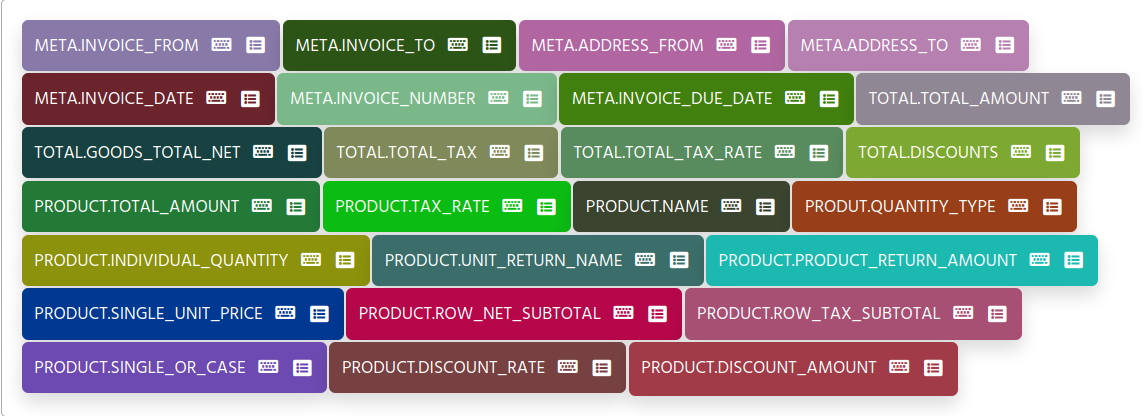
\includegraphics[width=0.9\textwidth]{figures/training_labels.png}
		      \caption{Training and Inference Labels created for the system.}
		      \label{fig:training_labels}
	      \end{figure}
		  \newpage
	\item \textbf{Annotation}: of all invoices in the dataset by applying the labels to the words. The annotation process is
	      very straightforward, the labels are color-coded and have customizable keyboard shortcuts. The text from the document
	      is OCR'd and displayed sequentially in the bottom half of the screen. The PDF document is displayed to the side.
	      One can simply highlight an area of text on the document and the current enabled label is applied to the text.
	      As text on the document is labeled the corresponding text is highlighted in the OCR'd output section.
	      \begin{figure}[H]
		      \centering
		      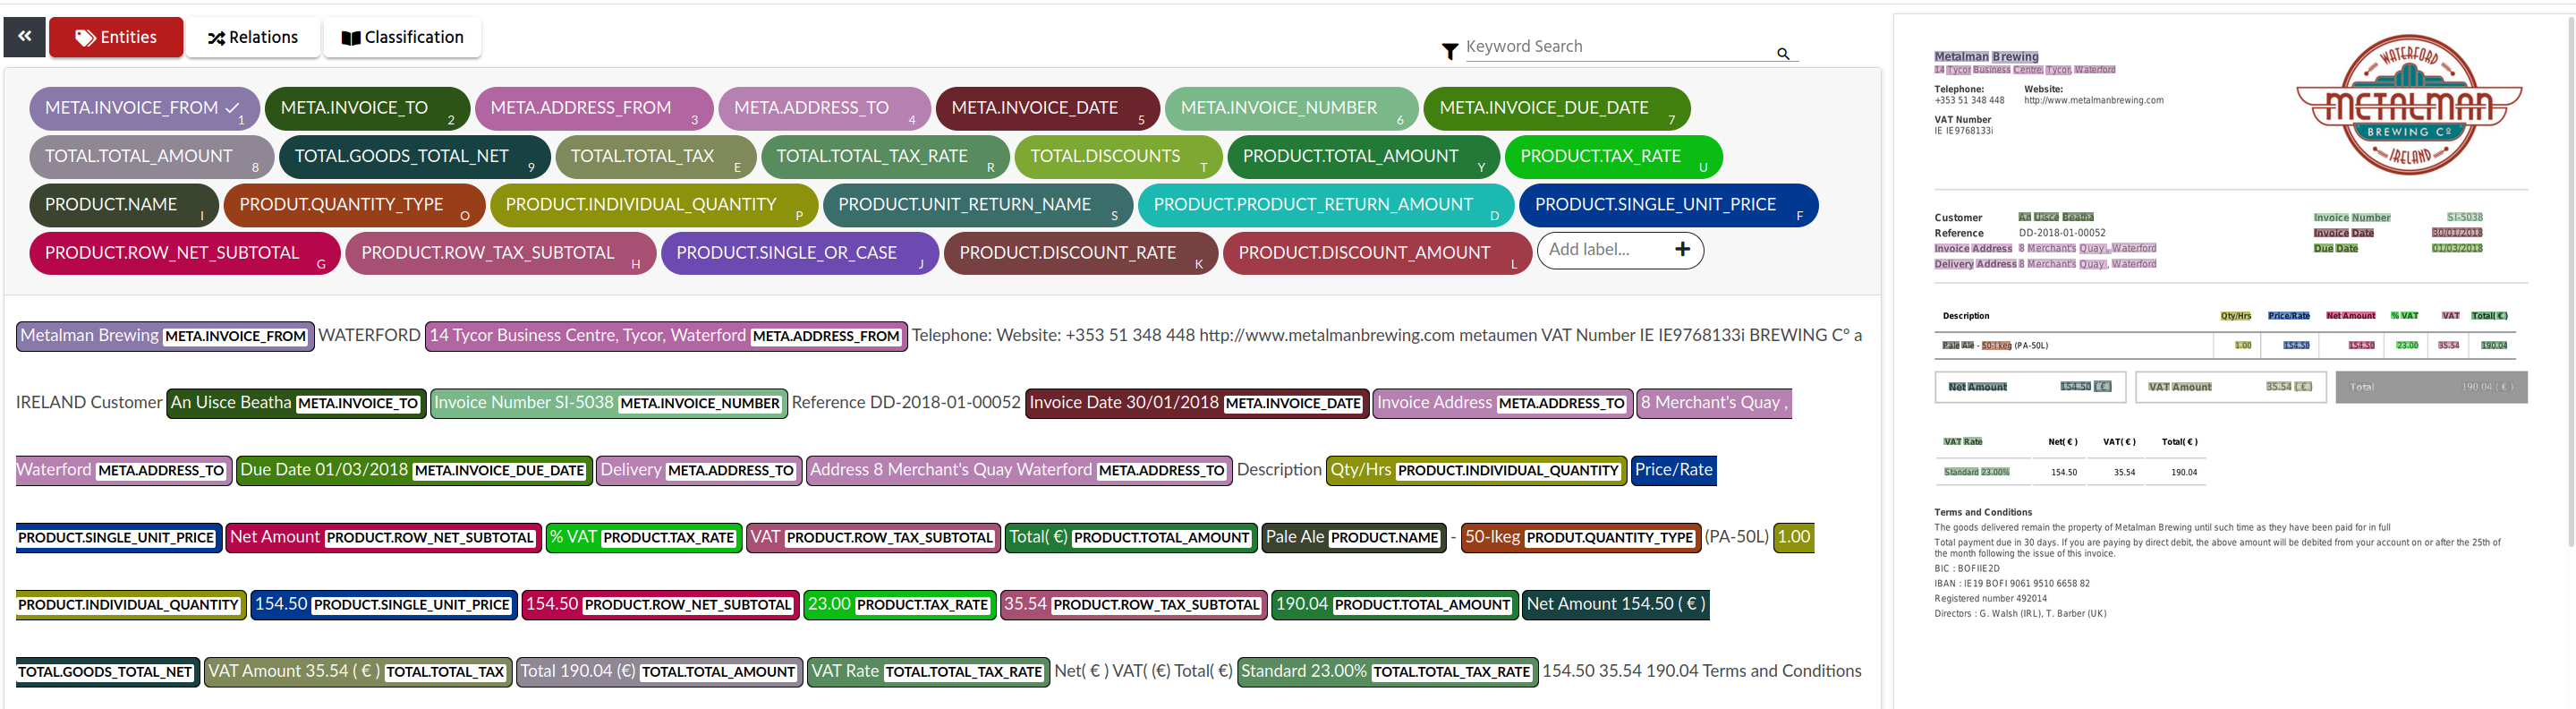
\includegraphics[width=1\textwidth]{figures/ubiai_annotate.png}
		      \caption{Annotating the dataset using UBIAI Annotation Tool.}
		      \label{fig:training_annotations}
	      \end{figure}
	      Even with this enhanced workflow, the annotation process was still very time-consuming. In total 86 documents
	      were annotated. Whilst this isn't an ideal amount, the larger the training set the better the model can
	      learn, research showed that from approximation. 50 documents LayoutLMv2 was able to return decent results.
	      This finding was corroborated by Walid.
	      \newpage
	      A further example of an annotated document is shown below.
	      \begin{figure}[H]
		      \centering
		      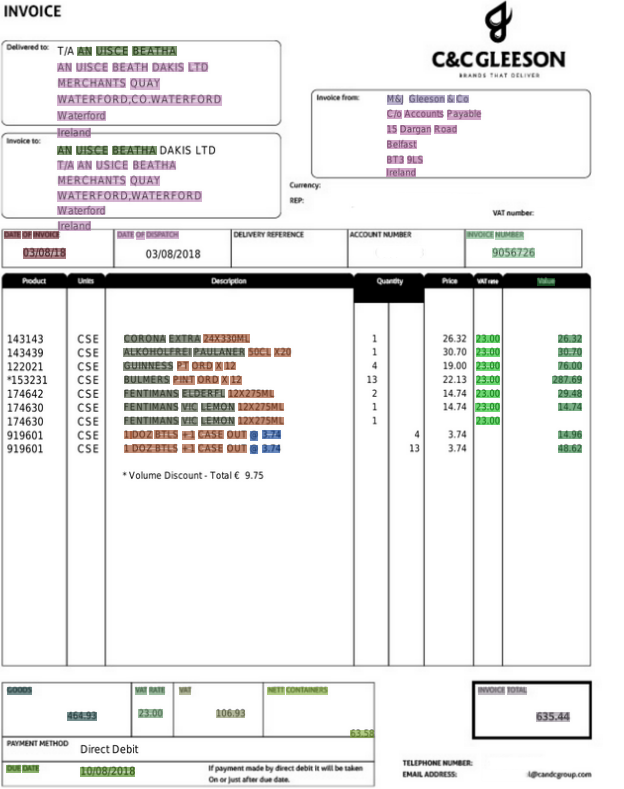
\includegraphics[width=1\textwidth]{figures/annotation_example.png}
		      \caption{Annotated example of a document.}
		      \label{fig:ubiai_annotate_example}
	      \end{figure}
	      \newpage

	\item \textbf{Exporting the Data}: the data is exported from the UBIAI software in an optimized format for the transformers
	      based architecture model. There appears to be a wide range of different options for data. With UBIAI supporting these methods:
	      \begin{figure}[H]
		      \centering
		      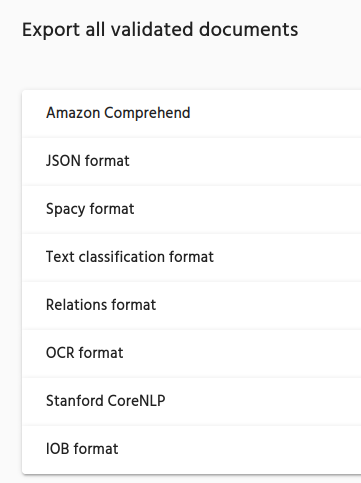
\includegraphics[width=0.35\textwidth]{figures/ubiai_export_options.png}
		      \caption{UBIAI Export Options.}
		      \label{fig:ubiai_export_options}
	      \end{figure}
	      If the data is not exported in the correct format it can take a large amount of time to transform the data into a
	      suitable format for the model.
	      The documents are exported along with some metadata files which contain the labels and the bounding boxes for each
	      document.
	      \bigbreak
	      The data is saved to Google drive so that it can be used in Google Colab along with being able to run locally. The model
	      was actually trained on Colab due to issues with the GPU memory on the development machine.
\end{enumerate}
% \begin{wrapfigure}{r}{0.35\textwidth}
% 	\centering
% 	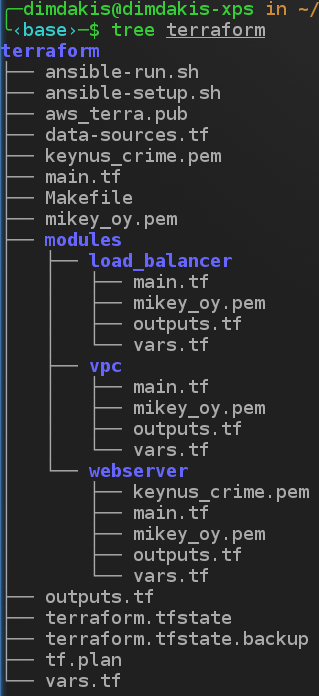
\includegraphics[width=0.3\textwidth]{figures/terra_dir_struct.png}
% 	\caption{The Terraform project structure}
% 	\label{fig:terra_project_structure}
% \end{wrapfigure}
\section{Training the Model}
Hugging Face provide a number of excellent tutorials and guides on how to train models here~\autocite{FinetunePretrainedModel}, there are also
some excellent resources on the topic here~\autocite{amamouFineTuningTransformerModel2021} and
here~\autocite{amamouFineTuningLayoutLMV22022}\footnote{Neither of the first two articles focus on LayoutLMv2,
	the former article is a generic guide whilst the second article focuses on the original LayoutLM model. The third article
	does focus on LayoutLMv2 but was only released after this project finished implementing training. I know of it and mention it here
	as the writer of the blog is the same Walid as I had interacted with about the annotation software. We had talked about the
	training and compared evaluation, scoring and results, etc., LayoutLMv2 is about to go into production for UBIAI. This is some further
	proof that the architecture chosen for this project is production ready.}.
The training script is written in Python, and it utilizes a number of libraries.
Including the following:
\begin{itemize}
	\item \textbf{PyTorch}: the main framework for the model.
	\item \textbf{torchvision}: the library for image processing.
	\item \textbf{transformers}: the library for the model and processor.
	\item \textbf{Detectron2}: the library for object detection.
\end{itemize}
With the dataset annotated and imported into the training script, the next step is to process the
data into the exact form needed to train the model. The data is manipulated and a Pandas dataframe
is created as per~\Cref{fig:training_dataframe}:
\begin{figure}[H]
	\centering
	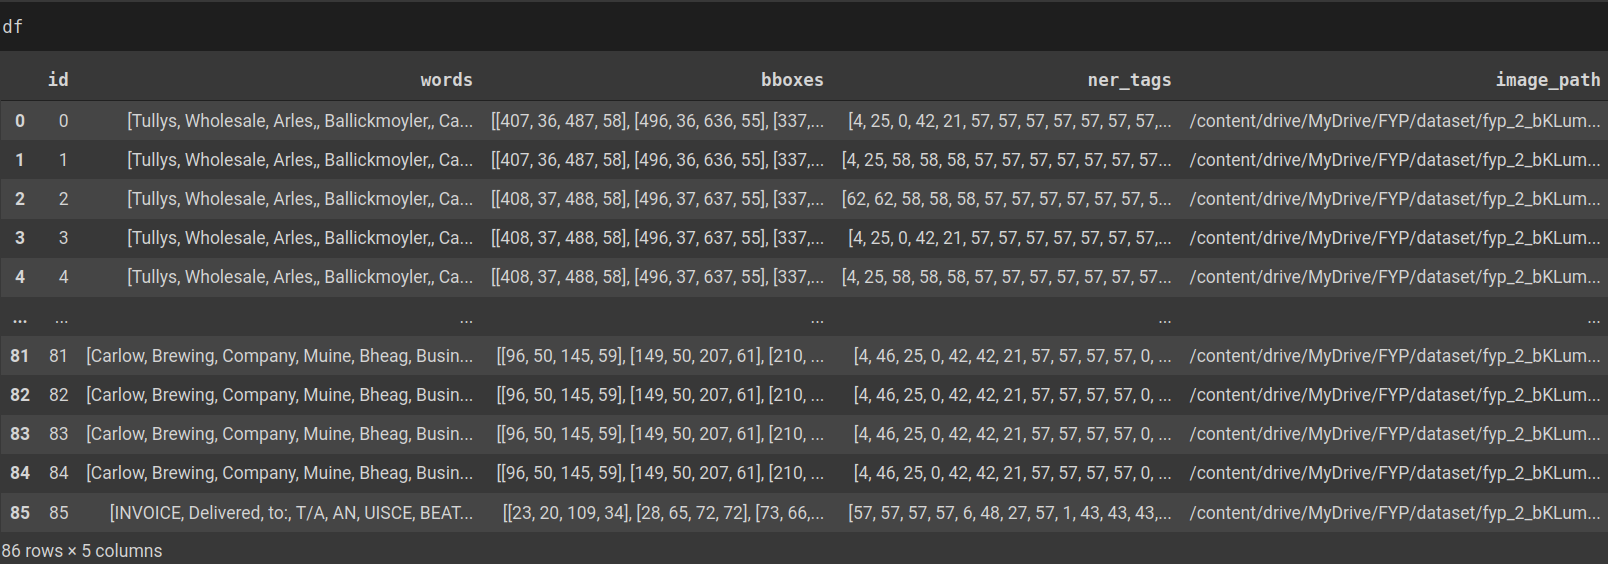
\includegraphics[width=1\textwidth]{figures/training_dataframe.png}
	\caption{Training Dataframe.}
	\label{fig:training_dataframe}
\end{figure}
It is important to note that each row in the dataframe represents a single document (invoice). For this training run,
there were 86 documents annotated, therefore, there are 86 rows in the dataframe. The columns are as follows:
\begin{itemize}
	\item \textbf{id}: The ID of the document, incrementing from 0 to 85.
	\item \textbf{words}: This is a list of every OCR'd word in the document, these words will be tokenized in the tokenizer
	      and form part of the input embedding.
	\item \textbf{bboxes}: This is a list of bounding boxes (the four coordinates of the box) for each word in the document.
	      the bounding boxes need to be normalized. This is done by dividing the bounding box coordinates by the width and height.
	      \begin{lstlisting}[language=python, label={lst:bbox_normalization}, caption={Bounding Box Normalization.}]
	def normalize_bbox(bbox, width, height):
    return [
        int(1000 * (bbox[0] / width)),
        int(1000 * (bbox[1] / height)),
        int(1000 * (bbox[2] / width)),
        int(1000 * (bbox[3] / height)),
    ]
	\end{lstlisting}
	\item \textbf{ner\_tags}: the Named Entity Relation (NER) tags for each word in the document. These are the labels
	      that were applied to the words. There is some minor processing done, to get to this stage. The labels are
	      encoded as integers and any word that doesn't have a label is assigned the label `0'.
	      \bigbreak
	      There are now more labels than were present initially. This is due to the giving the model some extra information,
	      where each prefix letter has a meaning. This meaning corresponds to the token position of the token in an entity.\\
	      The token prefixes are as follows:
	      \begin{itemize}
		      \item \textbf{B}: Beginning of a new entity.
		      \item \textbf{I}: Inside an entity. For example, the `State' token is a part of an entity like `Empire State Building`.
		            this means the ner\_tag would have a prefix of \code{I\_}~\autocite{TokenClassification}
		      \item \textbf{S}: This denotes a single token entity.
		      \item \textbf{E}: The token is the end of an entity.
		      \item \textbf{O}: Doesn't correspond to any entity.
	      \end{itemize}
	      These labels are then saved in the data\_config class which will be passed to the model during training and reused
	      for inference.
	      \begin{lstlisting}[language=python, label={lst:data_config}, caption={Data Config.}]
class data_config:
  labels = np.unique([tag for doc_tag in ner_tags for tag in doc_tag]).tolist()
  num_labels = len(labels)
  id2label = {v: k for v, k in enumerate(labels)}
  label2id = {k: v for v, k in enumerate(labels)}
	
\end{lstlisting}
	\item \textbf{image\_path}: the path to the image file. The tokenizer needs a copy of the image.
\end{itemize}

The amount of elements in the word, bboxes and ner\_tags columns should be equal.
\begin{figure}[H]
	\centering
	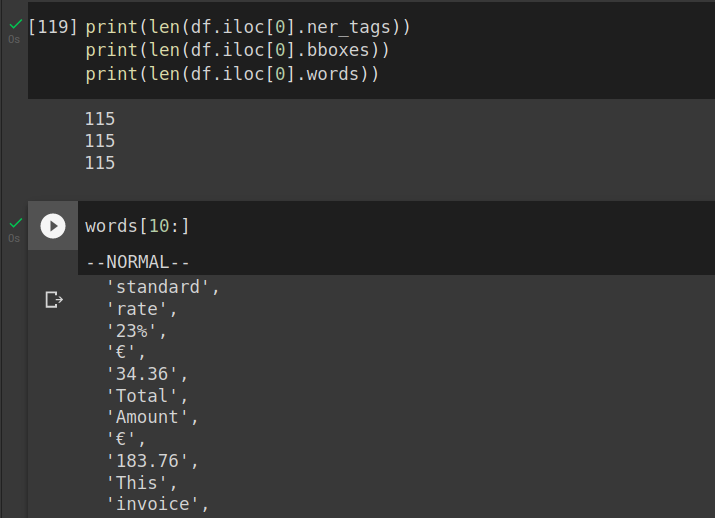
\includegraphics[width=0.6\textwidth]{figures/len_of_train_input.png}
	\caption{Sanity Check of the Length of the Training Input, can also see the words as input.}
	\label{fig:training_dataframe_columns}
\end{figure}
\bigbreak
\begin{itemize}
	\item The processor is downloaded from Hugging Face and the necessary inputs are passed in as parameters. Only the tokenizer part of the processor
	      is used.
	\item The datasets are then created using the Hugging Face Dataset function.
	\item The datasets are formatted.
\end{itemize}
\begin{lstlisting}[language=python, label={lst:dataset_creation}, caption={Dataset Preperation.}]
# processor download 
processor = LayoutLMv2Processor.from_pretrained("microsoft/layoutlmv2-base-uncased", revision="no_ocr")

# inputs that will become embeddings
encoded_inputs = processor(images, words, boxes=boxes, word_labels=word_labels,
                             padding="max_length", truncation=True)

# dataset creation
train_dataset = train_dataset.map(preprocess_data, batched=True, remove_columns=train_dataset.column_names,
                                      features=features)
valid_dataset = valid_dataset.map(preprocess_data, batched=True, remove_columns=valid_dataset.column_names,
                                      features=features)

# GPU settings for training
train_dataset.set_format(type="torch", device="cuda")
valid_dataset.set_format(type="torch", device="cuda")
\end{lstlisting}
The LayoutLMv2 model in this project is used in \emph{TokenClassification} mode. It will try
to classify each token in the invoice as belonging to a label category.\\
The model must be downloaded and fed the configurations.
\newpage
\begin{lstlisting}[language=python, label={lst:model_creation}, caption={Model Creation.}]
model_path = 'microsoft/layoutlmv2-base-uncased'

# config creation
config = LayoutLMv2Config.from_pretrained(model_path, num_labels=data_config.num_labels, id2label=data_config.id2label, label2id=data_config.label2id)

# model instantiation
model = LayoutLMv2ForTokenClassification.from_pretrained(model_path, config=config)

# model to CUDA, if available
model.to(device)
\end{lstlisting}

Now that the data is ready, and the model is created and configured the training function must be defined. It takes in
the training data, the model and the optimizer, in this case AdamW, as parameters:
\begin{lstlisting}[language=python, label={lst:train_function}, caption={Training Function.}]
def train_fn(train_dataloader, model, optimizer):
    total = len(train_dataloader)
    tk0 = tqdm(train_dataloader, total=total)
    train_loss = 0.0
    for bi, batch in enumerate(tk0):
        # embedding components
        input_ids = batch['input_ids'].to(device)
        bbox = batch['bbox'].to(device)
        attention_mask = batch['attention_mask'].to(device)
        token_type_ids = batch['token_type_ids'].to(device)
        labels = batch['labels'].to(device)
        resized_images = batch['image'].to(device)
        # forward pass
        outputs = model(image=resized_images, input_ids=input_ids, bbox=bbox, attention_mask=attention_mask, token_type_ids=token_type_ids, labels=labels)
        # loss and optimize
        loss = outputs.loss
        train_loss += loss.item()
        loss.backward()
        optimizer.step()
        # zero the parameter gradients for next iteration
        optimizer.zero_grad()
    return train_loss / total
\end{lstlisting}
This training function is then called in a loop. To match this with traditional learning 
the number of calls to this function would correspond to the number of epochs. 
\begin{figure}[H]
	\centering
	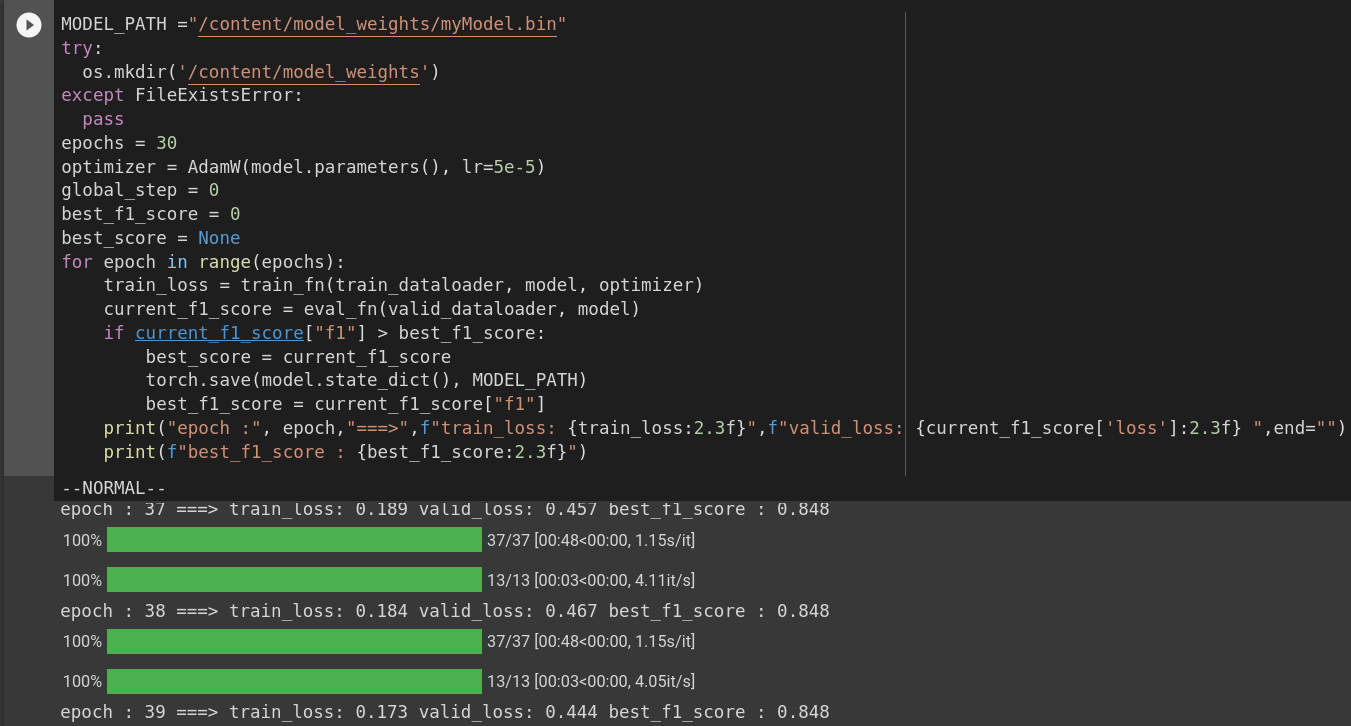
\includegraphics[width=1\textwidth]{figures/call_training_show_output.png}
	\caption{Calling Training Function, output of training depicting training loss, validation loss, epoch number
		and \FO\ score.}
	\label{fig:call_training_show_output}
\end{figure}
\subsection{Model Evaluation}
The default metric in a classification problem is the accuracy, due to its simplicity,
which is the fraction of correct predictions relative to the total number of predictions.
However, there are many situations in which this metric is unsuitable, for example when a dataset is imbalanced or,
as in this case, where our interest is in the positive cases only --- within this document did we identify/tag 
the relevant regions. In this situation, a more appropriate metric is the \FO\ score / metric.
To explain the \FO\ score~\autocite{mohajonConfusionMatrixYour2021},
the \emph{Confusion Matrix}\footnote{The example depicted is a simple binary confusion matrix,
	the actual confusion matrix for this model will have an $n * n$ matrix, where \emph{n}
	is the number of labels.} must be defined:
\begin{figure}[H]
	\centering
	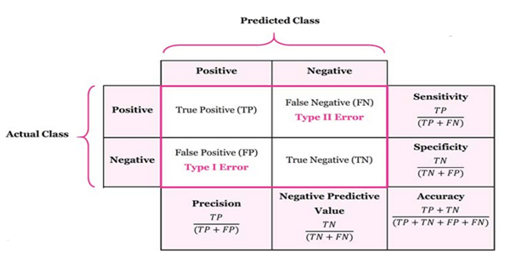
\includegraphics[width=0.8\textwidth]{figures/ml_scoring.png}
	\caption[Formulas for scoring]{Formulas for scoring sourced from here~\autocite{leeConfusionMatrixPrecision2021}.}
	\label{fig:f1_score_show_output}
\end{figure}
As can be seen in \Cref{fig:f1_score_show_output}, the confusion matrix is essentially built by comparing the model's
predictions (inference) and the actual values of the data. The formula for the \FO\ score is::
\[
	\FO =
	\frac{2}{\frac{1}{\text{Precision}} + \frac{1}{\text{Recall}}}
	=
	2 \times \frac{\text{Precision} \times \text{Recall}}{\text{Precision} + \text{Recall}}
	=
	\frac{2\times {TP} }{2\times{TP}+{FP}+{FN}}
\]
As the formula depends on \emph{Precision} and \emph{Recall} scores, first they must be defined:
\begin{itemize}
	\item \textbf{Precision}: Taking every prediction from the model, where that prediction is positive,
	      precision counts the percentage that is correct~\autocite{korstanjeF1Score2021}. Therefore,
		  \begingroup\smaller
	      \[
		      \text{Precision} =
		      \frac{\text{Number of True Positives ($TP$)}}
		      {\text{Number of True Positives ($TP$)} + \text{Number of False Positives ($FP$)}}
		      =
		      \frac{ {TP} }{{TP}+{FP}}
	      \]\endgroup
	      \begin{itemize}
		      \item A model with a low precision score may find many positives, but it also wrongly detects
		            many \emph{false positives} - positive predictions that are not actually positive.
		      \item A model with a high precision score may only find a few positives but from those that it predicts,
		            it correctly identifies a high percentage of them.
	      \end{itemize}
	\item \textbf{Recall}: Taking every true positive value\footnote{In this case, the actual labels as annotated in the
		      data preparation phase.} how many of these values did the model succeed in capturing~\autocite{korstanjeF1Score2021}. Therefore,
		  \begingroup\smaller
	      \[
		      \text{Recall} =
		      \frac{\text{Number of True Positives ($TP$)}}
		      {\text{Number of True Positives ($TP$)} + \text{Number of False Negatives ($FN$)}}
		      =
		      \frac{ {TP} }{{TP}+{FN}}
	      \]\endgroup
	      \begin{itemize}
		      \item A model with a low recall score may not find all, or a large proportion of the positive cases.
		      \item A model with a high recall score will discover a high proportion of the positive cases in the dataset but may also wrongly
		            identify some negative cases as positive cases.
	      \end{itemize}
\end{itemize}
Now that Precision and Recall are defined, the \FO\ score is a \emph{harmonic mean}~\autocite{HarmonicMean2022} of the two.
This returns the two scoring metrics as a single value, without having a bias toward one or the other, although this
can be shifted if the model use case cares more for one or the other.
\bigbreak
As can be observed from \Cref{fig:call_training_show_output}, the \FO\ score is coming in 84.8\%. This figure needs to be put into
context. What this figure actually means is that in terms of the documents, 84\% of the documents have been classified correctly.
This would mean that 84\% of the documents need not be classified. There would be some overhead in manually validating the
invoices. But the visual check of a document is a quicker process than the manual extraction. 
\section{Inference}
The next step is to test the model on data that it has not seen before. For this step an invoice must be OCR'd.
This is done in an API call to AWS Textract which returns OCR data in the following format:
\begin{figure}[H]
	\centering
	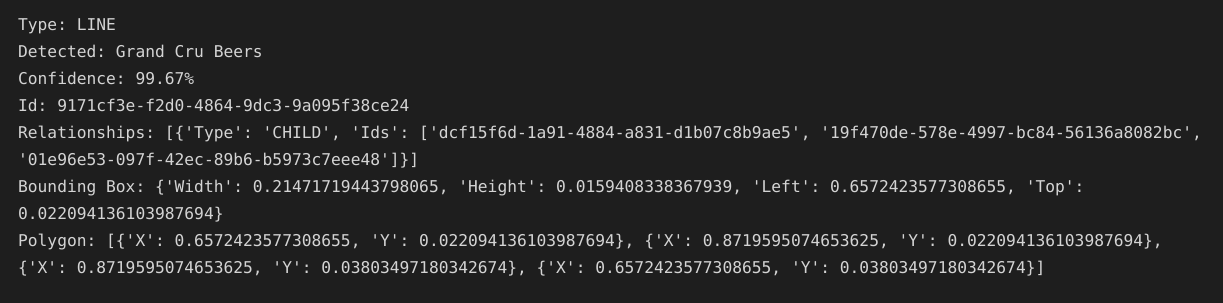
\includegraphics[width=1\textwidth]{figures/textract_output.png}
	\caption{Output of Textract API call, the boxes are the bounding boxes of the words in the invoice.}
	\label{fig:textract_output}
\end{figure}
Some pre-inference processing is required to prepare the data for the model. This step is similar to the data preparation
for training step. The tokenizer needs:
\begin{itemize}
	\item \textbf{words}: A list of all the words in the invoice.
	\item \textbf{bboxes}: The corresponding bounding boxes for each word.
	\item \textbf{image}: A copy of the image.
\end{itemize}
\newpage
\begin{lstlisting}[language=python, caption={Perperation for inference.}, label=prep_for_inference]
# define the tokenizer
inference_processor = LayoutLMv2Processor.from_pretrained("microsoft/layoutlmv2-base-uncased", revision="no_ocr")

# initializing the tokenizer with the correct data
inf_encoding = inference_processor(test_im, words, boxes=nbox,return_tensors="pt", padding="max_length", truncation=True) 

# map all tensors, inputs which will become embeddings, to cuda device
for k,v in inf_encoding.items():
  inf_encoding[k] = v.to(device)

# load the pre-trained model
model= torch.load(model_path,map_location=device)
\end{lstlisting}
Once these steps have been completed, the next step is inference.
\begin{lstlisting}[language=python, caption={Inference.}, label=inference]
# put the model in inference mode
model.eval()

# make the inference
with torch.no_grad():
  inference_outputs = model(**inf_encoding)
  #Output Logits (just before applying softmax)

#sanity check to check for shape
inference_outputs.logits.shape
\end{lstlisting}
Some post-processing is essential to make sense of the models output:
\begin{lstlisting}[language=python, caption={Inference Output Post-processing.}, label=infer_out_post_processing]
# remove CLS,PAD,and SEP special tokens from input text
raw_input_ids = inf_encoding['input_ids'][0].tolist()
# these are the predictions
predictions = inference_outputs.logits.argmax(-1).squeeze().tolist()
token_boxes = inf_encoding.bbox.squeeze().tolist()
special_tokens = [inference_processor.tokenizer.cls_token_id, inference_processor.tokenizer.sep_token_id, inference_processor.tokenizer.pad_token_id]

# conver the labels from their numerical lookup table value to the actual word
input_ids = [id for id in raw_input_ids if id not in special_tokens]
predictions = [model.config.id2label[prediction] for i,prediction in enumerate(predictions) if not (raw_input_ids[i] in special_tokens)]
actual_boxes = [unnormalize_box(box, width, height) for i,box in enumerate(token_boxes) if not (raw_input_ids[i] in special_tokens )]
\end{lstlisting}
The predictions contains a list of labels for each word in the input. Words which do not fit any labels are denoted with an `O'. These
are stripped out in the final part of the post-processing. 
With the inference complete, the labels are drawn on to the image to visually show the results.
\begin{figure}[H]
	\centering
	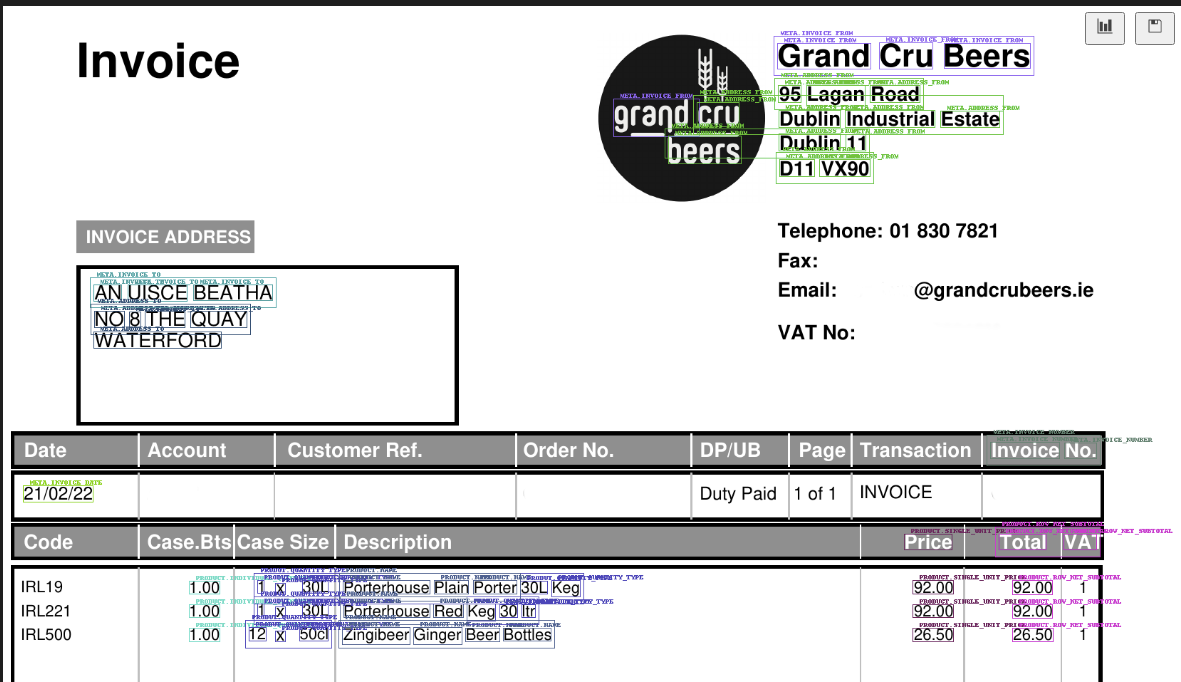
\includegraphics[width=1\textwidth]{figures/inf_example_top.png}
	\caption{Example 1 of the inference, bounding boxes around the words with the corresponding labels inferred by the model.}
	\label{fig:inference_output_top}
\end{figure}
Just based upon an informal visual inspection of the invoice, we can see the model is performing well.
% list out things it got right
A further example of the output that is, currently, of most interest to the project:
\begin{figure}[H]
	\centering
	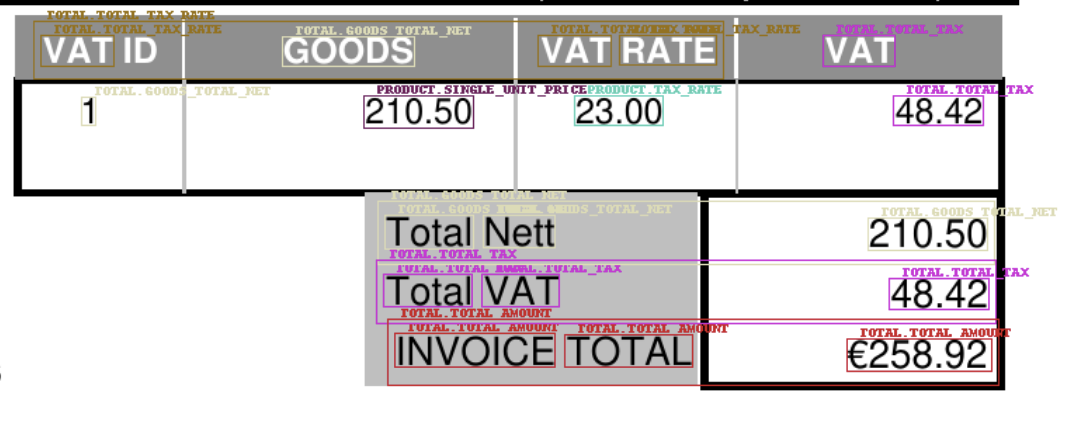
\includegraphics[width=0.9\textwidth]{figures/infer_example_bottom.png}
	\caption{Example 2 output of the inference, the boxes are the bounding boxes of the words in the invoice, with the corresponding labels
		inferred by the model.}
	\label{fig:inference_output_bottom}
\end{figure}
The model has correctly identified all the totals that are of interest. This leaves less post-processing to do to obtain
the final results ready for the database. 

\subsection{Post-Processing}
After this some validation checks and further manipulation of the output data is carried out. The checks include the following:
The total amount of the invoice is labelled and is correct. This can done by checking the total amount figures are present. 
If there is no total amount, then the system will look to create it from the net and vat amounts.
The validation added has meant that with every tested invoice thus far, the system has correctly identified all the figures that
are of interest.
\section{Exposing the Pipeline as a REST API}
The pipeline consists of 20 functions which make up the entire pre-process, inference, post-process and saving to database in Kubernetes phases.
To expose the pipeline as a REST API, a server must be initialized:
\begin{lstlisting}[language=python, caption={Initializing the Server.}, label=server_init]
# initialize the server
app = Flask(__name__)
# configurations for server
app.config.from_pyfile('config.cfg')

# setting the logger
log.getLogger('sqlalchemy.dialects.postgresql').setLevel(log.INFO)

# initialising metrices for prometheus monitoring
metrics = PrometheusMetrics(app)
metrics.info('app_info', 'Application info', version='0.0.1')

# custom metrics
REQUESTS = Counter("http_requests_total", "HTTP requests")
IN_PROGRESS = Gauge("inprogress_requests", "Inprogress HTTP requests",
        multiprocess_mode='livesum')
REQUEST_TIME = Summary('request_processing_seconds', 'Time spent processing request')
\end{lstlisting}
\textbf{Note}: Even though the server is running locally, there is some additional code such as the Prometheus metrics in \Cref{server_init}
which are specific to a Kubernetes deployment. As the initial development had been done to run the pipeline in the Kubernetes
cluster, metrics and specialized logging are present in the code. The Inference Server is \emph{Kubernetes-ready}.
\begin{lstlisting}[language=python, caption={Inference Endpoint Defined.}, label=infer_endpoint]
@app.route('/invoiceLocation', methods=['GET', 'POST'])
def invoiceLocation():
	# NUM_REQUESTS.inc()
	if request.method == 'POST':
		# get the document
		document = request.form['document']
		# get the bucket name
		bucket_name = request.form['bucket_name']

		# start the pipeline
		model = load_model(model_path)
		inference_processor = load_inference_processor()
		iServe = InferenceServer(model_path)
		print('loaded model and inference processor')
		print(f'bucket_name = {bucket_name}, document = {document}')
		print ('starting pipeline')
		# timing the pipline run
		start_time = datetime.time()
		# run the pipeline
		filtered_words = InferenceServer.start_pipeline(document, bucket_name, model, inference_processor)
		end_time = datetime.time()
		print(f'Pipeline completed in: {end_time - start_time}')
		# return the filtered words
		return jsonify(filtered_words)
	else:
		return jsonify({'error': 'no document'})
	
\end{lstlisting}
The last step then is to start the server:
\begin{lstlisting}[language=python, caption={Starting the Server.}, label=server_start]
if __name__ == '__main__':
	load_dotenv()

	logging.basicConfig(level=os.environ.get("LOGLEVEL", "INFO"))
	# instantiate logger object
	log = logging.getLogger(__name__)

	# register_metrics(app, app_version="v0.1.2", app_config="stage")
	dispatcher = DispatcherMiddleware(app.wsgi_app, {"/metrics": make_wsgi_app()})
	run_simple(hostname="localhost", port=5000, application=dispatcher)
\end{lstlisting}
\section{Gmail Scraper}
The Gmail server is a Python CLI application which is used to scrape the Gmail inbox, searching for invoices. There is nothing
earth-shattering here. If the reader wants to see the code it is present in the code repository.
\section{ML Pipeline Performance}
Pipeline run time:
\begin{figure}[H]
	\centering
	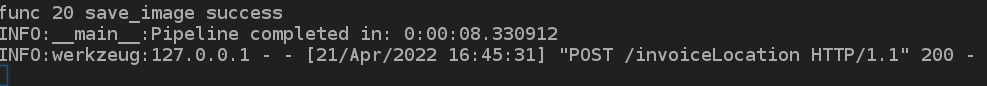
\includegraphics[width=0.9\textwidth]{figures/pipeline_time.png}
	\caption{Timing of the pipeline run time.}
	\label{fig:pipeline_run_time}
\end{figure}
As can be seen the entire pipeline takes a mere 8 seconds to run. This includes AWS interaction,
pre- and post-processing, and saving to database. This is a very satisfying result and is proof that efficiency was at front and
center focus during the development of the project.

